%% ============================================================
%% RQ1_Presentation.tex
%% Domain Shift in HAR: WISDM vs UCI HAR
%% Beamer presentation — compile with pdflatex
%% ============================================================
\documentclass[aspectratio=169, 10pt]{beamer}

%% ── Theme ────────────────────────────────────────────────────
\usetheme{Madrid}
\usecolortheme{beaver}
\usefonttheme{professionalfonts}
\setbeamertemplate{navigation symbols}{}          % hide nav icons
\setbeamertemplate{caption}[numbered]
\setbeamersize{text margin left=6mm, text margin right=6mm}

%% ── Packages ─────────────────────────────────────────────────
\usepackage{graphicx}
\usepackage{booktabs}
\usepackage{tabularx}
\usepackage{array}
\usepackage{xcolor}
\usepackage{tikz}
\usepackage{amsmath}
\usepackage{multicol}
\usepackage{colortbl}

%% ── Graphics path ────────────────────────────────────────────
\graphicspath{{figures/}}

%% ── Custom colours ───────────────────────────────────────────
\definecolor{wisdmOrange}{RGB}{224, 123, 57}
\definecolor{uciBlue}{RGB}{58, 125, 201}
\definecolor{alertRed}{RGB}{180, 30, 30}
\definecolor{noteGray}{RGB}{100, 100, 100}
\definecolor{highlightYellow}{RGB}{255, 245, 180}
\definecolor{darkRed}{RGB}{140,0,0}

%% ── Helper commands ──────────────────────────────────────────
\newcommand{\wisdm}{\textcolor{wisdmOrange}{\textbf{WISDM}}}
\newcommand{\uci}{\textcolor{uciBlue}{\textbf{UCI HAR}}}
\newcommand{\metricbox}[2]{%
  \begin{beamercolorbox}[sep=3pt,center,rounded=true,shadow=false]{block body}
    \textbf{#1}\\[2pt]\large #2
  \end{beamercolorbox}}

%% ── Title info ───────────────────────────────────────────────
\title[Domain Shift in HAR]{Domain Shift in Human Activity Recognition}
\subtitle{A Quantitative Analysis of WISDM vs.\ UCI HAR}
\author{RQ1 Technical Analysis}
\institute{Sensor Data Analytics / Machine Learning Systems}
\date{March 2026}

%% ============================================================
\begin{document}

%% ── Title slide ──────────────────────────────────────────────
\begin{frame}
  \titlepage
  \vspace{-4mm}
  \begin{center}
    \small\textcolor{noteGray}{
      \textbf{Research Question:} \emph{What are the key sources of domain shift across
      the WISDM dataset and other HAR datasets?\\
      What metrics can be used to quantify the differences?}}
  \end{center}
\end{frame}

%% ── Outline ──────────────────────────────────────────────────
\begin{frame}{Outline}
  \tableofcontents[hideallsubsections]
\end{frame}

\section{Motivation}
\section{Dataset Overview}
\section{Methodology}
\section{Results}
\section{Conclusions}

%% ============================================================
%%  SECTION 1 — MOTIVATION
%% ============================================================

\begin{frame}{Why Does Domain Shift Matter in HAR?}
  \begin{columns}[T]
    \begin{column}{0.52\textwidth}
      \textbf{The deployment gap}
      \begin{itemize}
        \item Models trained on dataset A fail on dataset B — even for the \emph{same} activity classes
        \item Accuracy can drop from \textbf{95\%} (within-dataset) to \textbf{$<$60\%} (cross-dataset)
        \item Root cause is rarely understood at the signal level
      \end{itemize}

      \vspace{4mm}
      \textbf{Why WISDM and UCI HAR?}
      \begin{itemize}
        \item Two of the \textbf{most widely cited} HAR benchmarks
        \item Nominally identical task: 6-class accelerometer HAR
        \item Yet they embody \emph{fundamentally different} data-generating processes
      \end{itemize}
    \end{column}

    \begin{column}{0.44\textwidth}
      \begin{block}{The Core Question}
        \centering
        \vspace{2mm}
        \emph{What exactly makes these datasets different — and how do we \textbf{measure} it?}
        \vspace{2mm}
      \end{block}

      \vspace{4mm}
      \begin{alertblock}{Key Claim}
        Domain shift in HAR is \textbf{multi-source} and \textbf{anisotropic}.\\
        Scalar metrics (e.g.\ mean Acc Magnitude) hide the dominant shift axis.
      \end{alertblock}
    \end{column}
  \end{columns}
\end{frame}

%% ============================================================
%%  SECTION 2 — DATASET OVERVIEW
%% ============================================================

\begin{frame}{Dataset Overview — \wisdm\ vs.\ \uci}
  \begin{center}
  \small
  \begin{tabularx}{0.95\textwidth}{lXX}
    \toprule
    \textbf{Property} & \textcolor{wisdmOrange}{\textbf{WISDM v1.1}} & \textcolor{uciBlue}{\textbf{UCI HAR}} \\
    \midrule
    Subjects            & 36                        & 30 \\
    Sampling rate       & 20 Hz                     & 50 Hz \\
    Sensor placement    & \textbf{Front trouser pocket} (free-swinging) & \textbf{Waist-mounted} (fixed) \\
    Sensors             & Accelerometer only        & Accelerometer \textbf{+ Gyroscope} \\
    Gravity separation  & \textbf{None} (raw total\_acc) & \textbf{Butterworth LPF} applied \\
    Activities          & Walk, \textbf{Jog}, Up, Down, Sit, Stand & Walk, Up, Down, Sit, Stand, \textbf{Lay} \\
    Total windows*      & 43,347                    & 8,355 \\
    Collection setting  & \textbf{In the wild}      & \textbf{Controlled lab} \\
    \bottomrule
    \multicolumn{3}{l}{\tiny * After alignment: 20 Hz, 51-sample (2.56 s) windows}
  \end{tabularx}
  \end{center}

  \vspace{2mm}
  \begin{columns}[T]
    \begin{column}{0.48\textwidth}
      \centering
      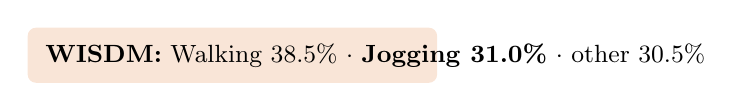
\begin{tikzpicture}
        \fill[wisdmOrange!20, rounded corners=3pt] (0,0) rectangle (5.2,0.7);
        \node[anchor=west] at (0.1, 0.35) {\small \textbf{WISDM:} Walking 38.5\% $\cdot$ \textbf{Jogging 31.0\%} $\cdot$ other 30.5\%};
      \end{tikzpicture}
    \end{column}
    \begin{column}{0.48\textwidth}
      \centering
      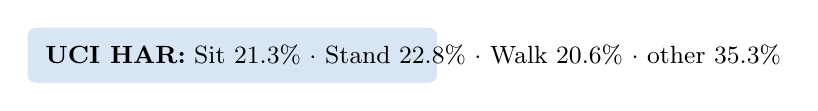
\begin{tikzpicture}
        \fill[uciBlue!20, rounded corners=3pt] (0,0) rectangle (5.2,0.7);
        \node[anchor=west] at (0.1, 0.35) {\small \textbf{UCI HAR:} Sit 21.3\% $\cdot$ Stand 22.8\% $\cdot$ Walk 20.6\% $\cdot$ other 35.3\%};
      \end{tikzpicture}
    \end{column}
  \end{columns}
\end{frame}

\begin{frame}{Label Space — Shared Activities and Gaps}
  \begin{columns}[T]
    \begin{column}{0.58\textwidth}
      \small
      \begin{tabularx}{\textwidth}{clcc}
        \toprule
        \textbf{ID} & \textbf{Unified Label} & \textcolor{wisdmOrange}{\textbf{WISDM}} & \textcolor{uciBlue}{\textbf{UCI}} \\
        \midrule
        0 & Walking    & \checkmark & \checkmark \\
        1 & \textbf{Jogging}   & \checkmark & \textcolor{alertRed}{\textbf{---}} \\
        2 & Upstairs   & \checkmark & \checkmark \\
        3 & Downstairs & \checkmark & \checkmark \\
        4 & Sitting    & \checkmark & \checkmark \\
        5 & Standing   & \checkmark & \checkmark \\
        --- & \textbf{Laying}  & \textcolor{alertRed}{\textbf{---}} & \checkmark \\
        \bottomrule
      \end{tabularx}
    \end{column}

    \begin{column}{0.38\textwidth}
      \begin{alertblock}{Activity Gap}
        \begin{itemize}
          \item \textbf{Jogging} occupies \textbf{31\%} of WISDM — no UCI counterpart
          \item \textbf{Laying} is UCI-only — dropped from analysis
          \item Irresolvable by any preprocessing
        \end{itemize}
      \end{alertblock}

      \vspace{3mm}
      \begin{block}{5 Shared Classes}
        Walk, Upstairs, Downstairs, Sitting, Standing
      \end{block}
    \end{column}
  \end{columns}
\end{frame}

%% ============================================================
%%  SECTION 3 — METHODOLOGY
%% ============================================================

\begin{frame}{Methodology Pipeline}
  \begin{center}
  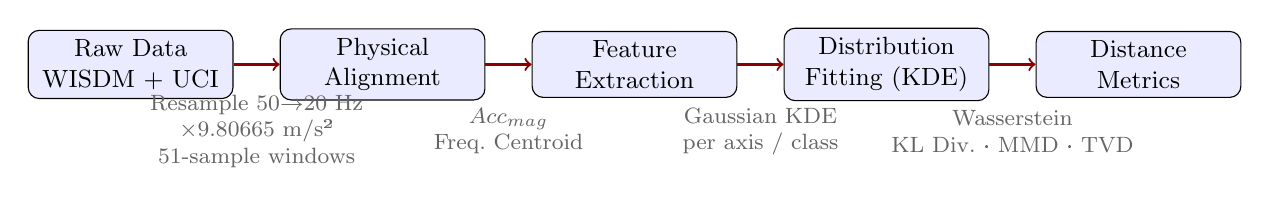
\begin{tikzpicture}[
      box/.style={draw, rounded corners=4pt, fill=blue!8, minimum width=2.6cm,
                  minimum height=0.8cm, font=\small, align=center},
      arrow/.style={->, thick, color=darkRed}
    ]
    \node[box] (raw)   at (0,0)   {Raw Data\\WISDM + UCI};
    \node[box] (align) at (3.2,0) {Physical\\Alignment};
    \node[box] (feat)  at (6.4,0) {Feature\\Extraction};
    \node[box] (dist)  at (9.6,0) {Distribution\\Fitting (KDE)};
    \node[box] (metr)  at (12.8,0){Distance\\Metrics};

    \draw[arrow] (raw)   -- (align);
    \draw[arrow] (align) -- (feat);
    \draw[arrow] (feat)  -- (dist);
    \draw[arrow] (dist)  -- (metr);

    \node[font=\footnotesize, text=noteGray, align=center] at (1.6,-0.85)
      {Resample 50$\to$20 Hz\\$\times$9.80665 m/s²\\51-sample windows};
    \node[font=\footnotesize, text=noteGray, align=center] at (4.8,-0.85)
      {$Acc_{mag}$\\Freq.\ Centroid};
    \node[font=\footnotesize, text=noteGray, align=center] at (8.0,-0.85)
      {Gaussian KDE\\per axis / class};
    \node[font=\footnotesize, text=noteGray, align=center] at (11.2,-0.85)
      {Wasserstein\\KL Div.\ · MMD · TVD};
  \end{tikzpicture}
  \end{center}

  \vspace{3mm}
  \begin{columns}[T]
    \begin{column}{0.48\textwidth}
      \textbf{Two extracted features per window:}
      \begin{itemize}
        \item \textbf{Acc Magnitude}: $Acc_{mag}(t) = \sqrt{x^2 + y^2 + z^2}$
        \item \textbf{Frequency Centroid}: $f_c = \frac{\sum f_i \cdot P(f_i)}{\sum P(f_i)}$
      \end{itemize}
    \end{column}
    \begin{column}{0.48\textwidth}
      \textbf{Four distance metrics:}
      \begin{itemize}
        \item Wasserstein-1 (EMD) — transport cost
        \item Symmetric KL Divergence — overlap
        \item Multi-kernel MMD — feature-space shift
        \item Total Variation Distance — prior shift
      \end{itemize}
    \end{column}
  \end{columns}
\end{frame}

%% ============================================================
%%  SECTION 4 — RESULTS
%% ============================================================

\begin{frame}{Results I — Physical Feature Distributions (Overview)}
  \begin{center}
    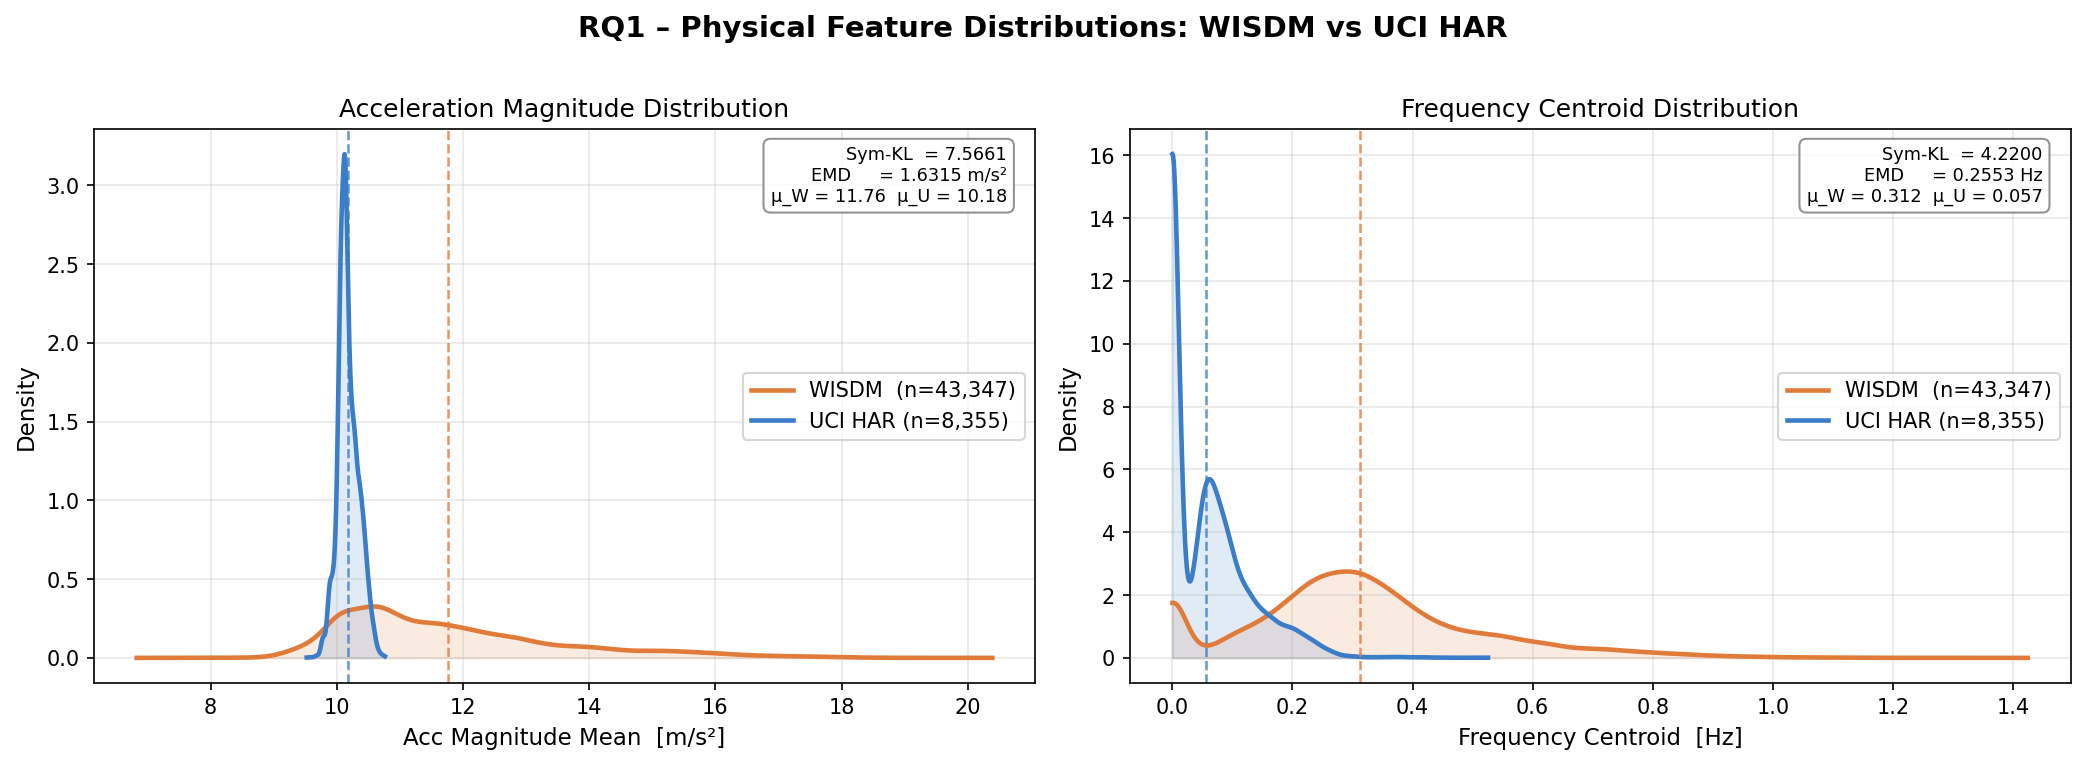
\includegraphics[width=0.88\textwidth, height=0.68\textheight, keepaspectratio]
      {RQ1_Physical_Distributions.png}
  \end{center}
  \vspace{-2mm}
  \begin{columns}[T]
    \begin{column}{0.48\textwidth}
      \small \textcolor{wisdmOrange}{$\bullet$} WISDM: broad, right-skewed \\
      \small \textcolor{uciBlue}{$\bullet$} UCI: narrow spike near 1$g$ = 9.81 m/s²
    \end{column}
    \begin{column}{0.48\textwidth}
      \small Frequency centroid gap: $\bar{f}_W = 0.312$ Hz vs.\ $\bar{f}_U = 0.057$ Hz \textbf{(5.5$\times$)}
    \end{column}
  \end{columns}
\end{frame}

\begin{frame}{Results II — Dominant Source: Sensor Orientation}
  \begin{center}
    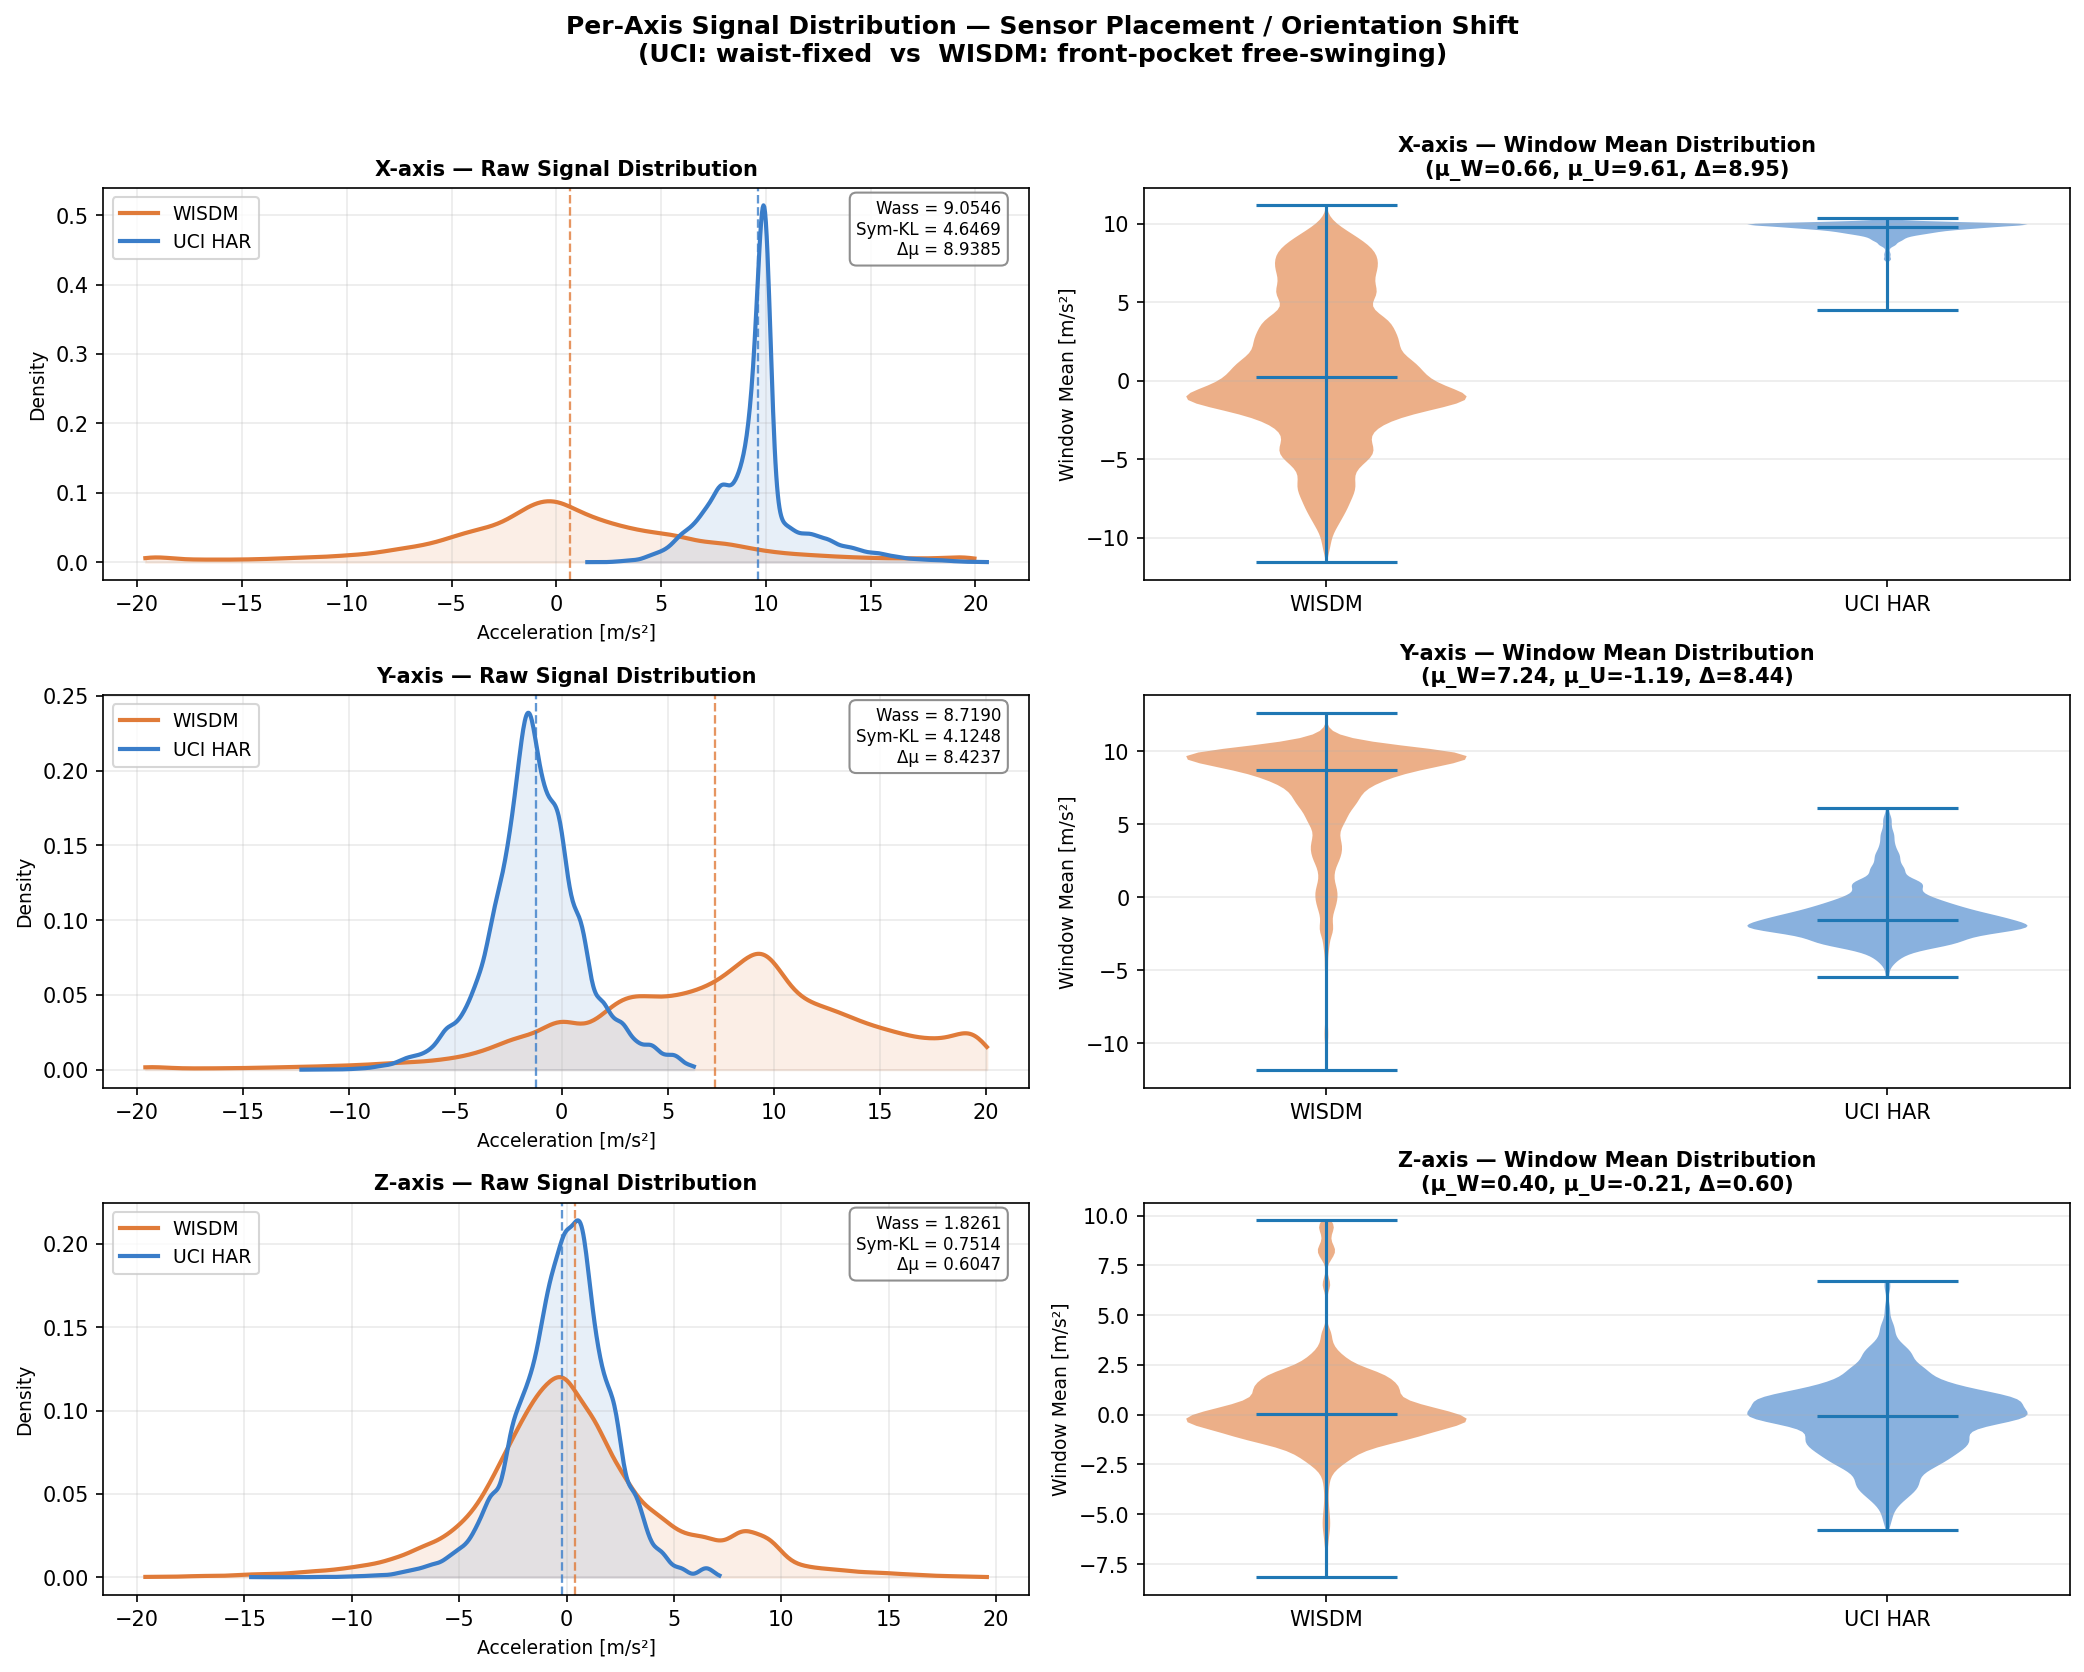
\includegraphics[width=0.92\textwidth, height=0.72\textheight, keepaspectratio]
      {per_axis_analysis.png}
  \end{center}
  \vspace{-2mm}
  \begin{center}
    \small \textbf{X-axis:} Wass = 9.06 m/s² \quad \textbf{Y-axis:} Wass = 8.72 m/s² \quad
    \textbf{Z-axis:} Wass = 1.83 m/s² \quad
    \textcolor{alertRed}{\textbf{$\gg$ Scalar Acc Mag = 1.63 m/s²}}
  \end{center}
\end{frame}

\begin{frame}{Results III — Gravity Component \& Preprocessing Gap}
  \begin{center}
    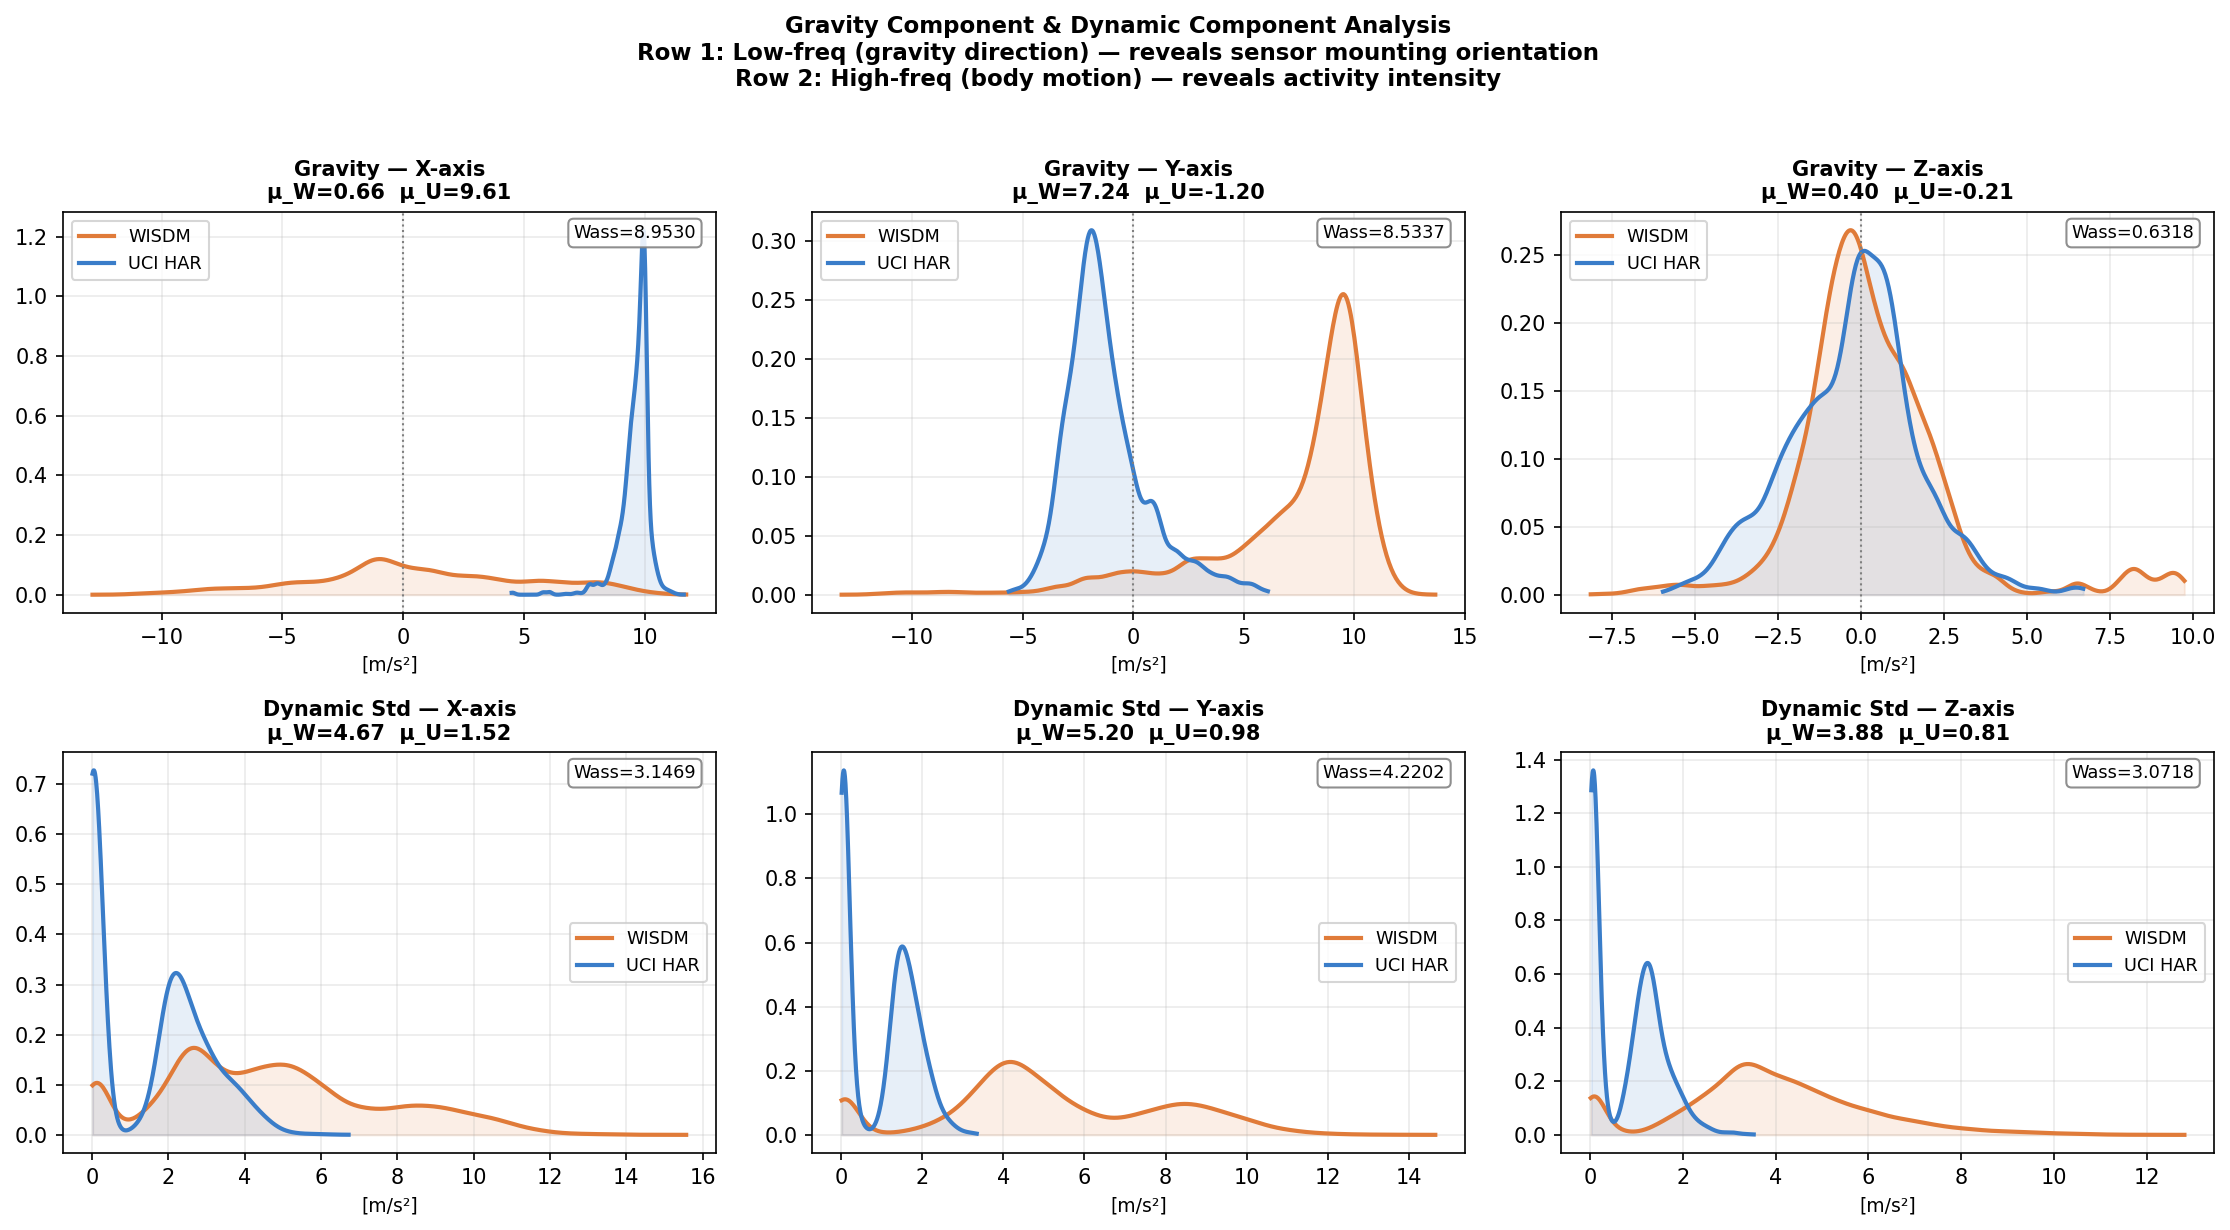
\includegraphics[width=0.90\textwidth, height=0.68\textheight, keepaspectratio]
      {gravity_bias_analysis.png}
  \end{center}
  \vspace{-2mm}
  \begin{columns}[T]
    \begin{column}{0.55\textwidth}
      \small \textbf{Row 1:} Gravity concentrates on \textbf{X} in UCI (+8.58), on \textbf{Y} in WISDM (+6.51) — sensor orientations near-orthogonal
    \end{column}
    \begin{column}{0.42\textwidth}
      \small \textbf{Row 2:} Dynamic std \textbf{3--5$\times$ higher} in WISDM; UCI applied Butterworth gravity separation
    \end{column}
  \end{columns}
\end{frame}

\begin{frame}{Results IV — Class Prior Shift $P(Y)$}
  \begin{center}
    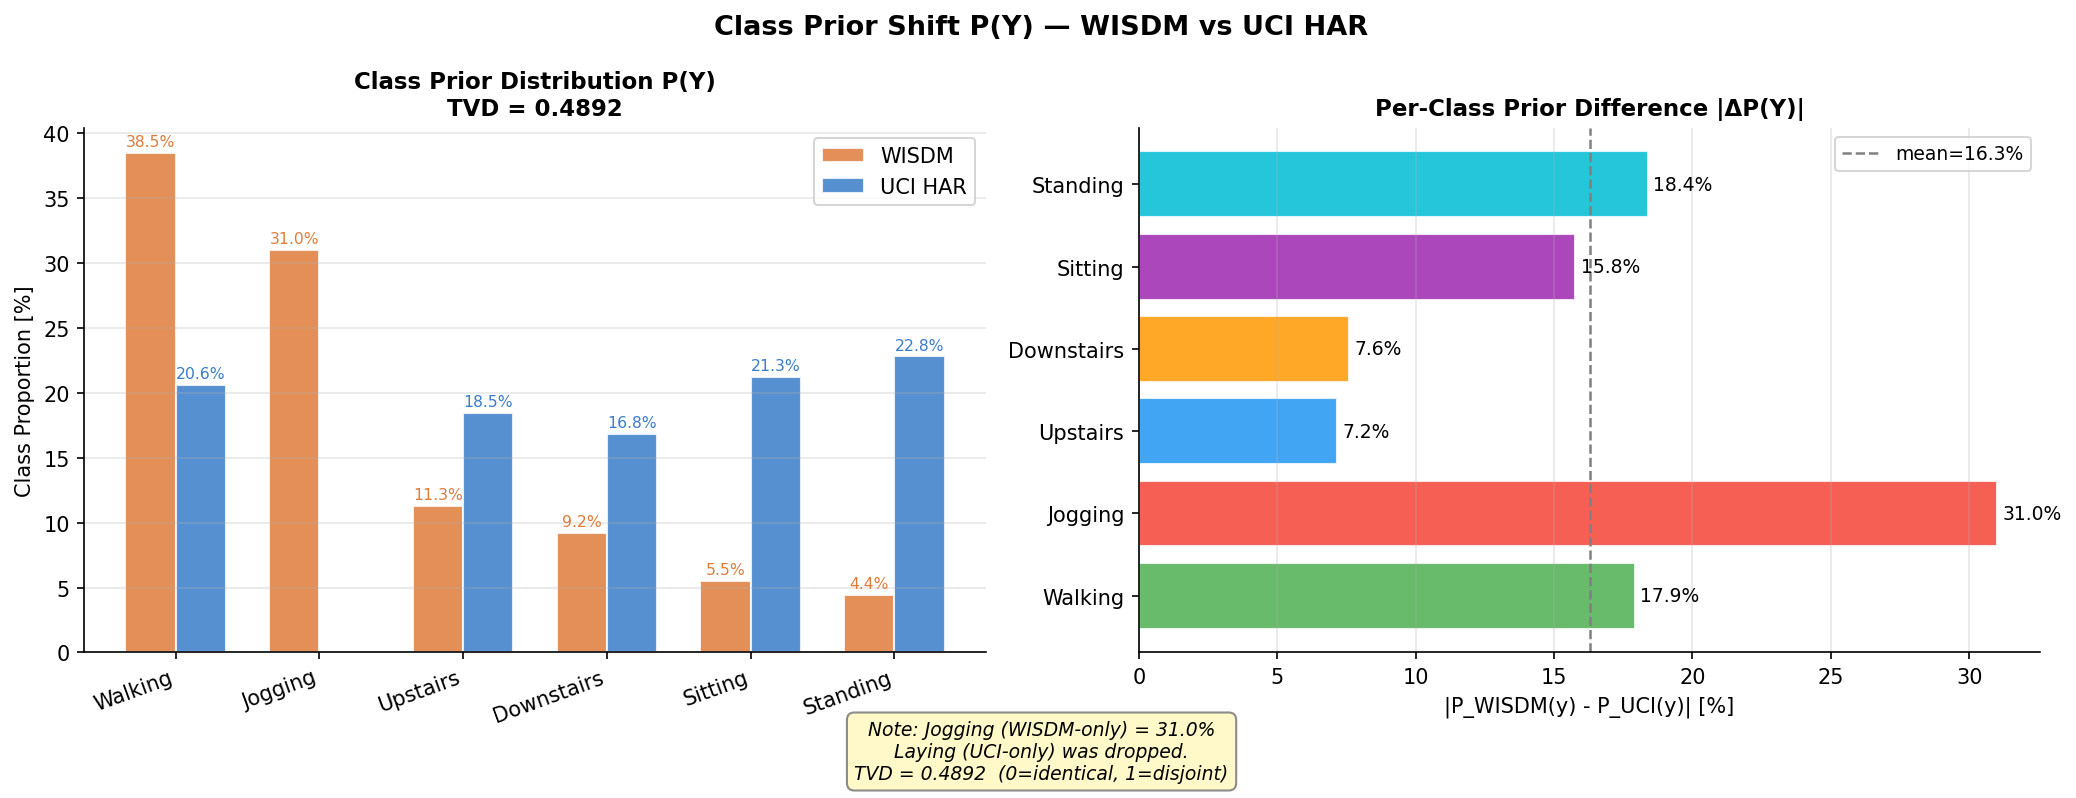
\includegraphics[width=0.88\textwidth, height=0.70\textheight, keepaspectratio]
      {class_prior_shift.png}
  \end{center}
  \vspace{-2mm}
  \begin{center}
    \small Total Variation Distance $\mathbf{TVD = 0.489}$ \quad
    Jogging: $\Delta P = 31.0\%$ \quad Standing: $\Delta P = 18.4\%$ \quad Walking: $\Delta P = 17.9\%$
  \end{center}
\end{frame}

\begin{frame}{Results V — Per-Class Covariate Shift}
  \begin{columns}[T]
    \begin{column}{0.50\textwidth}
      \centering
      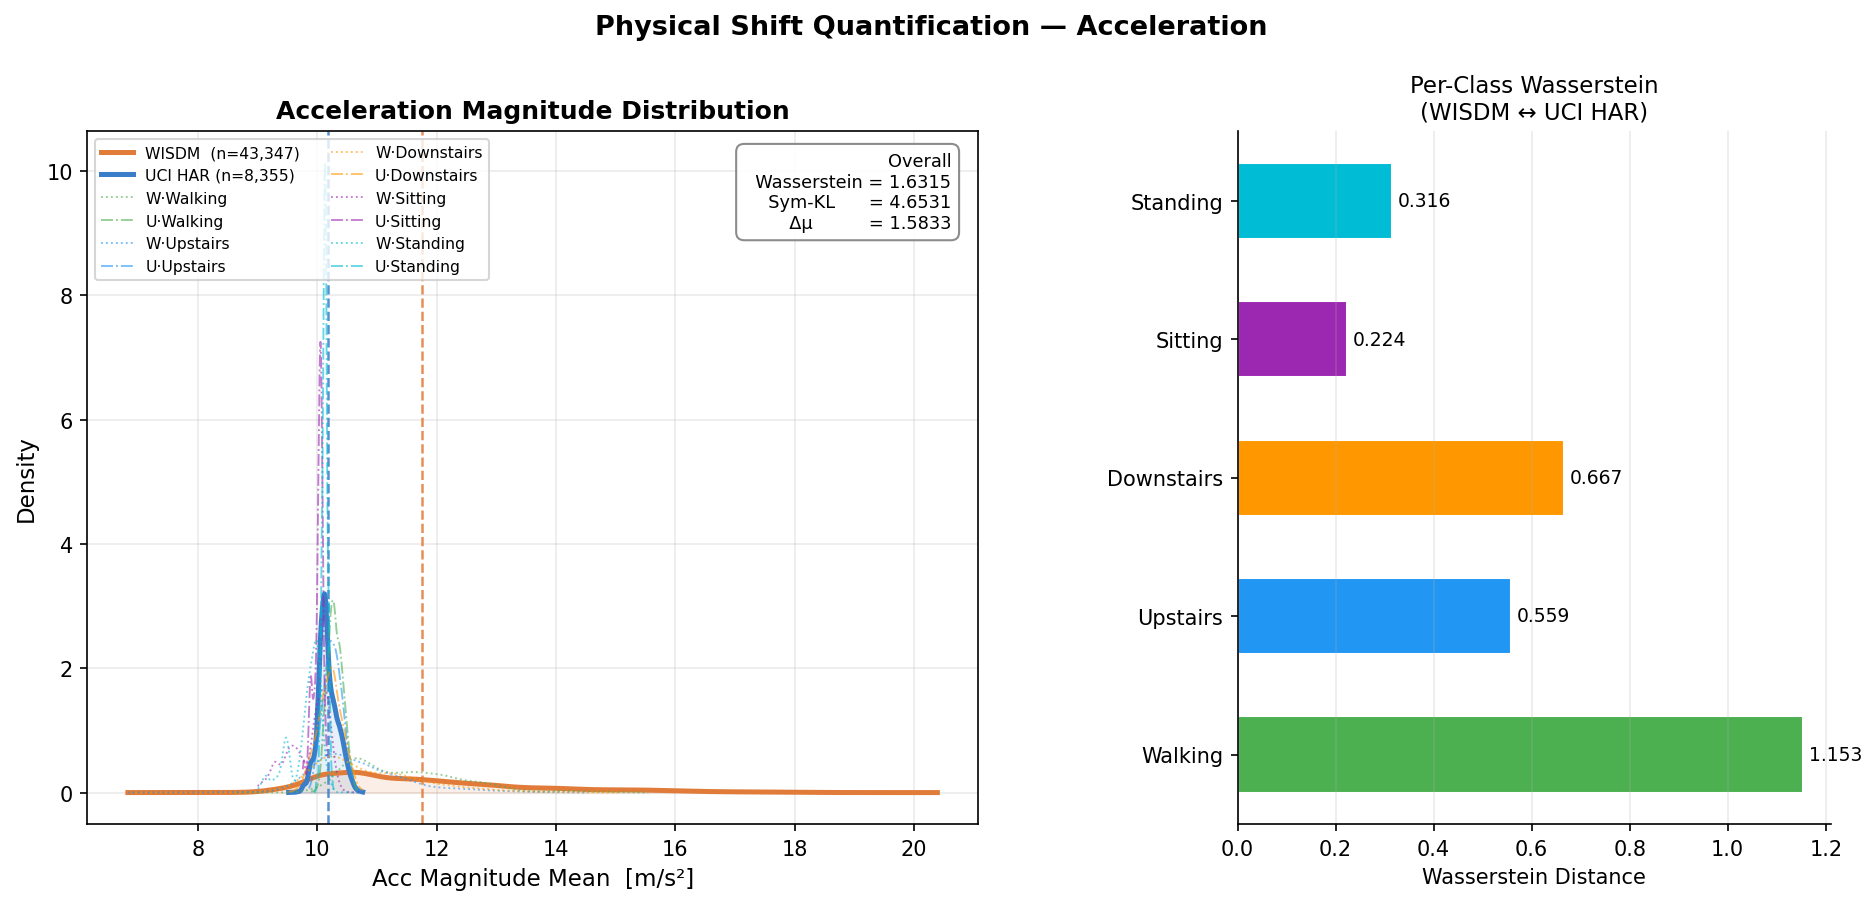
\includegraphics[width=\textwidth, height=0.68\textheight, keepaspectratio]
        {amplitude_dist_metrics.png}
      \\\small Acc Magnitude per class
    \end{column}
    \begin{column}{0.48\textwidth}
      \centering
      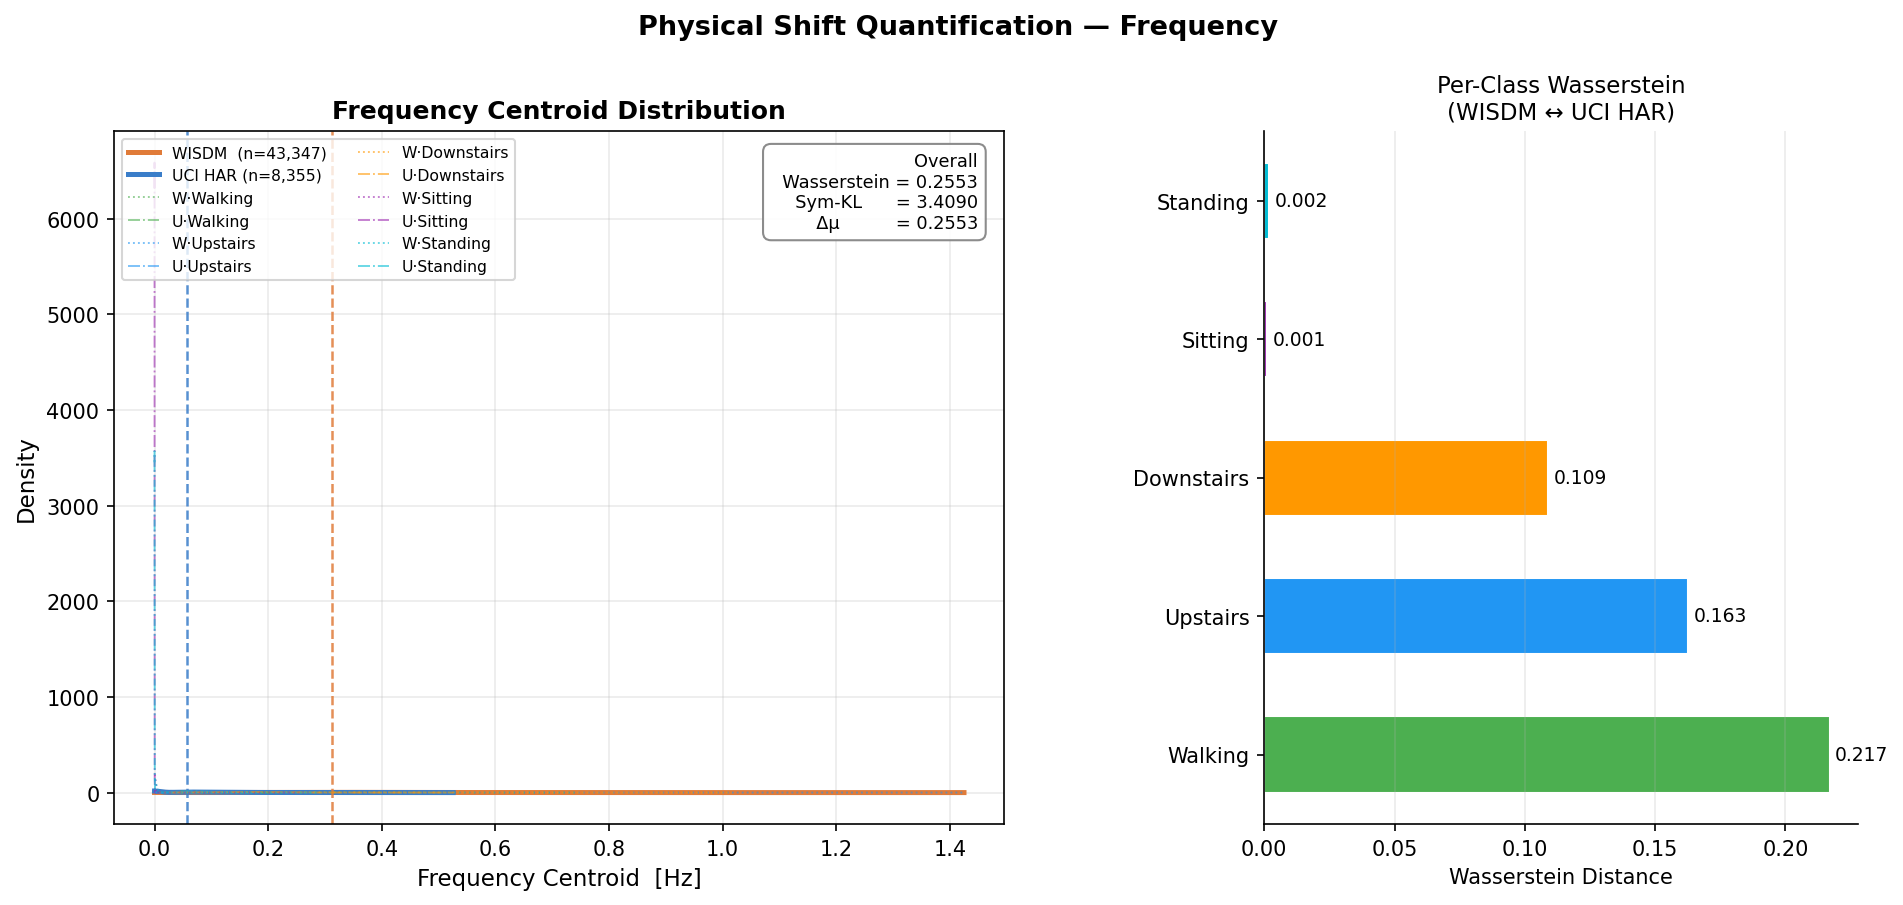
\includegraphics[width=\textwidth, height=0.68\textheight, keepaspectratio]
        {freq_centroid_dist_metrics.png}
      \\\small Frequency Centroid per class
    \end{column}
  \end{columns}
  \vspace{1mm}
  \begin{center}
    \small \textbf{Walking} has the largest per-class shift (Wass = 1.15 m/s²) \quad
    \textbf{Sitting/Standing} nearly aligned across datasets
  \end{center}
\end{frame}

\begin{frame}{Results VI — Feature Space Geometry (MMD)}
  \begin{center}
    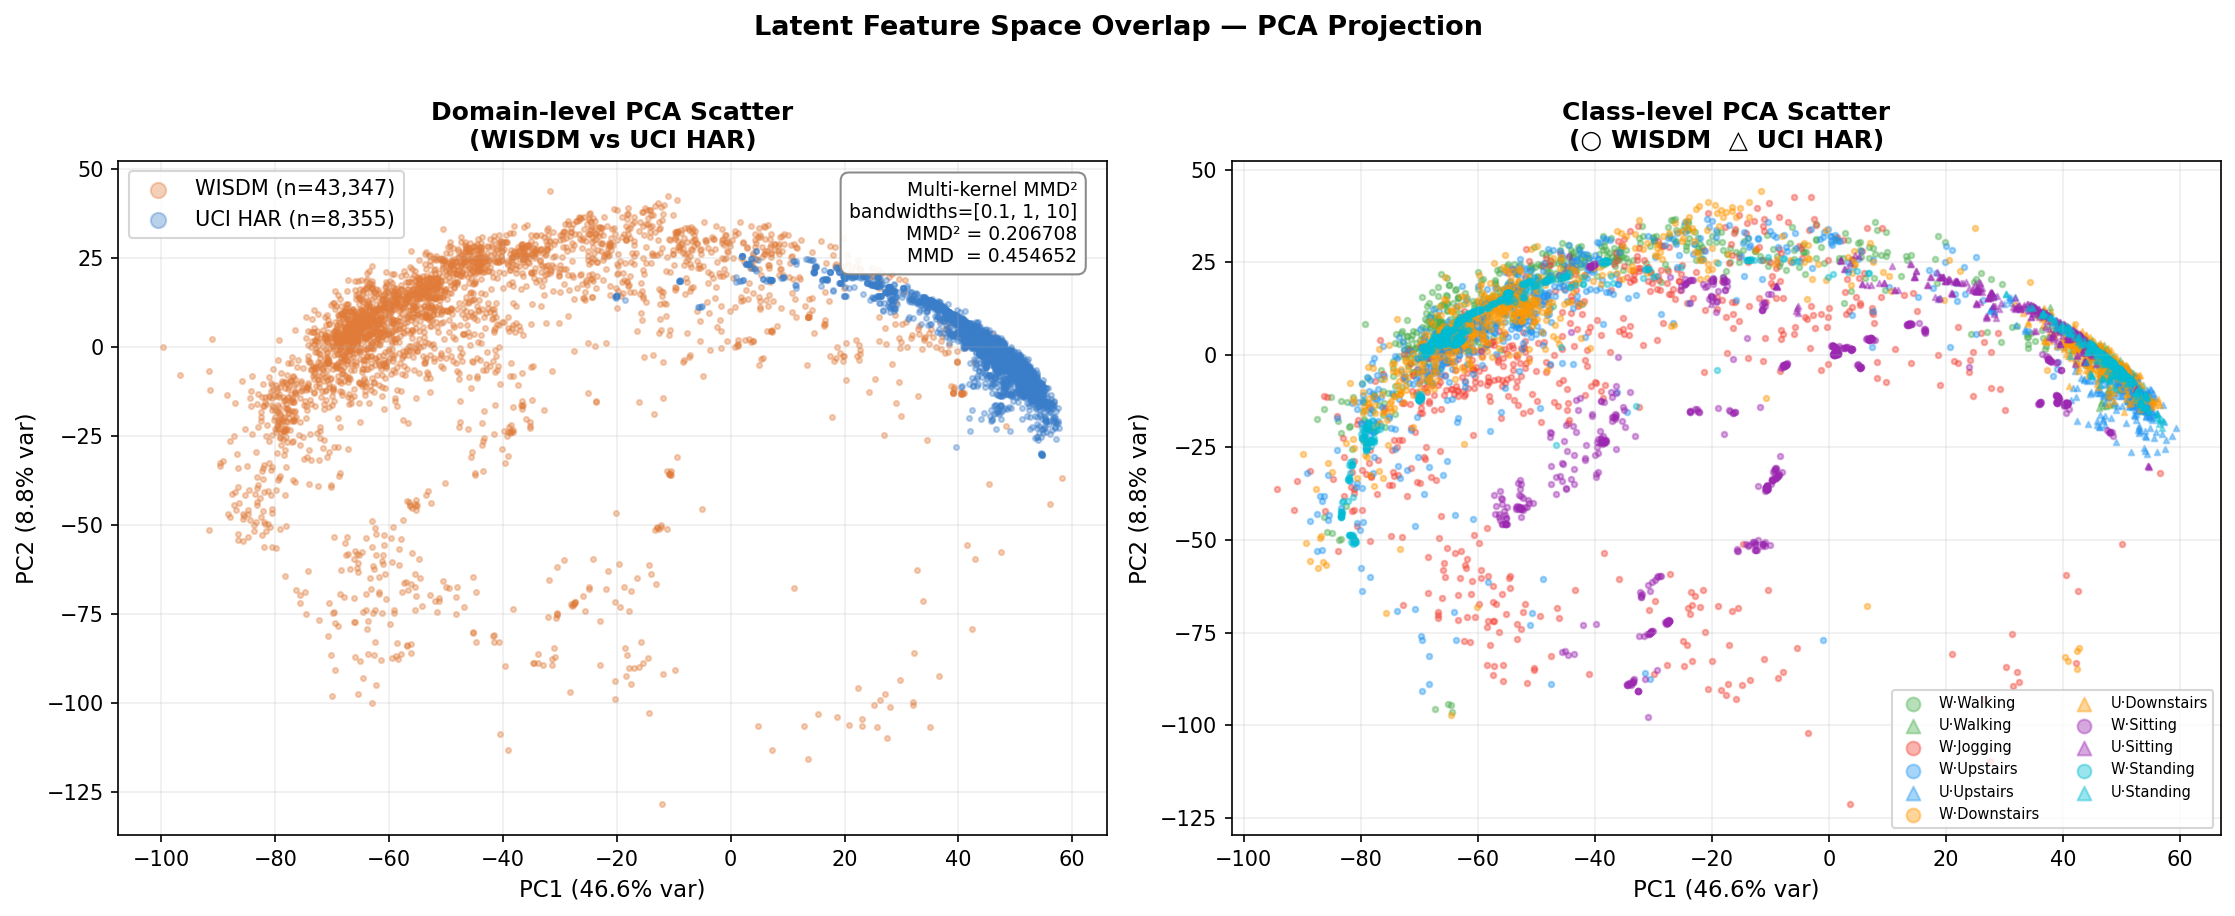
\includegraphics[width=0.88\textwidth, height=0.70\textheight, keepaspectratio]
      {latent_space_overlap.png}
  \end{center}
  \vspace{-2mm}
  \begin{center}
    \small
    \textbf{Multi-kernel MMD} (bandwidths 0.1, 1, 10): $\mathbf{MMD^2 = 0.2067}$,\; $\mathbf{MMD = 0.455}$
    \quad Left: domain-coloured \quad Right: class-coloured
  \end{center}
\end{frame}

\begin{frame}{Results VII — Inter-Subject Variability}
  \begin{columns}[T]
    \begin{column}{0.58\textwidth}
      \centering
      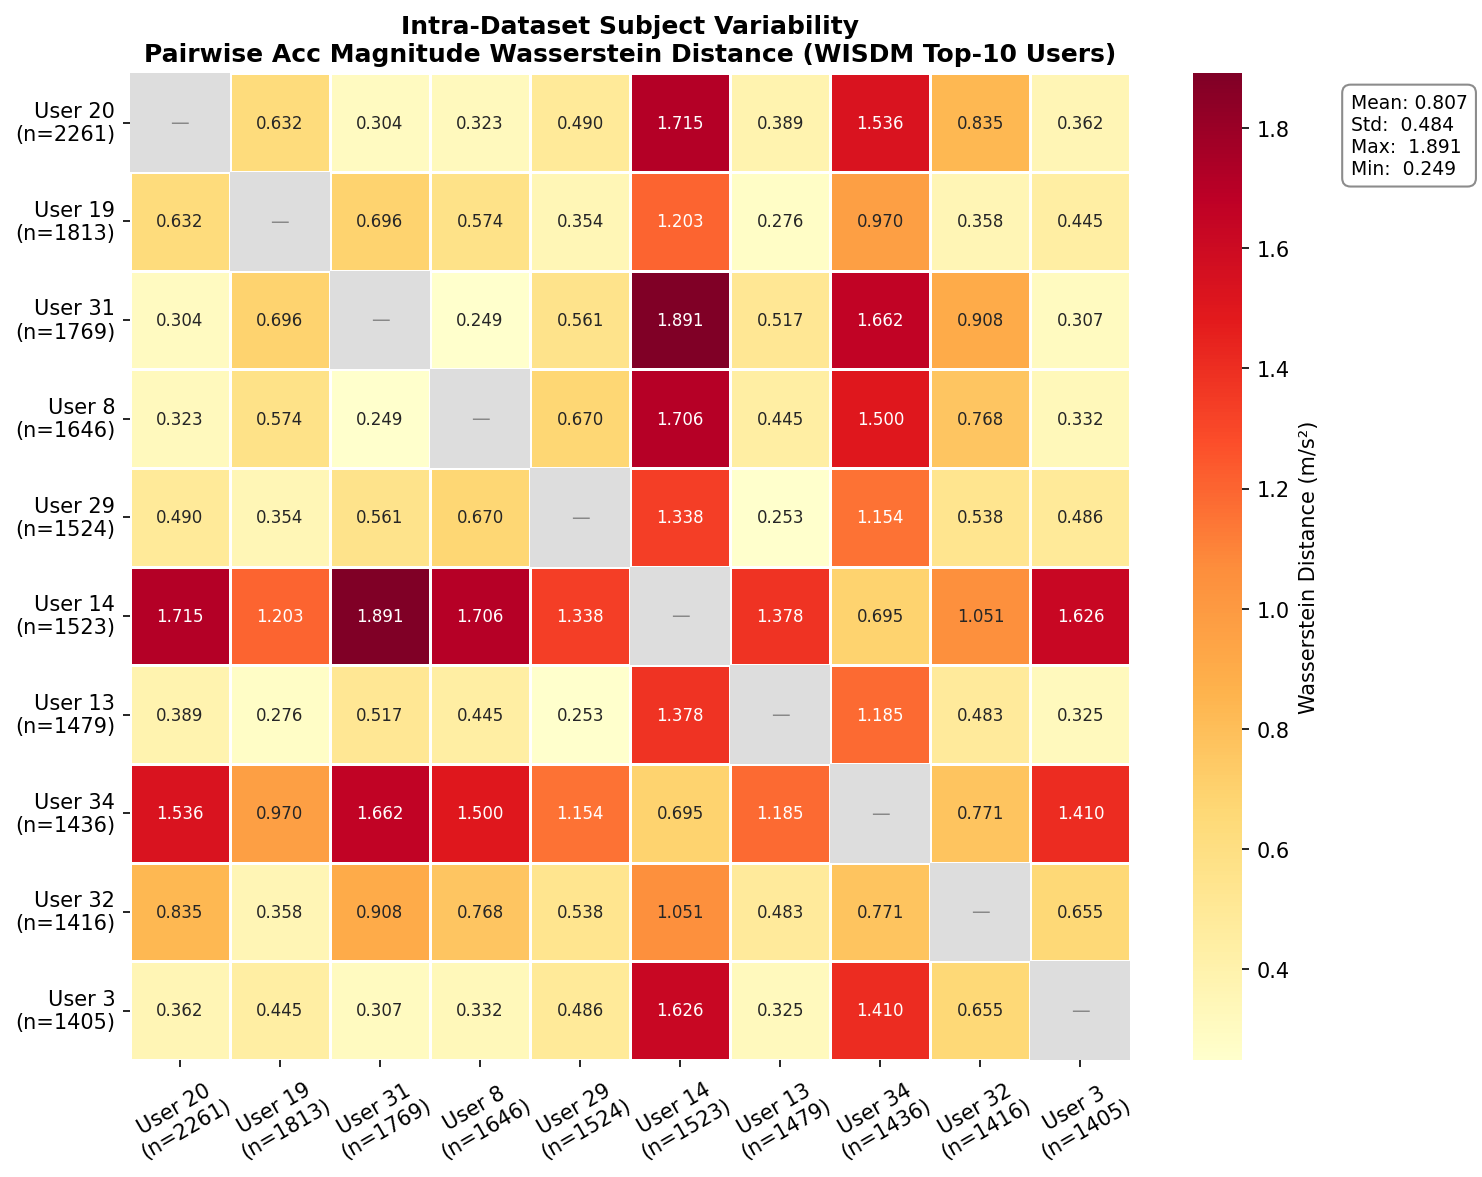
\includegraphics[width=\textwidth, height=0.72\textheight, keepaspectratio]
        {subject_wasserstein_heatmap.png}
    \end{column}
    \begin{column}{0.38\textwidth}
      \vspace{6mm}
      \begin{block}{Key Numbers}
        \small
        \begin{tabular}{lr}
          Mean intra-user Wass & 0.807 \\
          Max intra-user Wass  & \textbf{1.891} \\
          \midrule
          Cross-dataset Wass   & \textbf{1.631} \\
        \end{tabular}
      \end{block}

      \vspace{4mm}
      \begin{alertblock}{Critical Finding}
        \small Max user-pair distance \textbf{(1.89)} exceeds cross-dataset shift \textbf{(1.63)}.\\[3pt]
        Subject shift is \textbf{not secondary} — it is a first-class problem.
      \end{alertblock}
    \end{column}
  \end{columns}
\end{frame}

\begin{frame}{Results VIII — Gait Periodicity \& Spectral Analysis}
  \begin{center}
    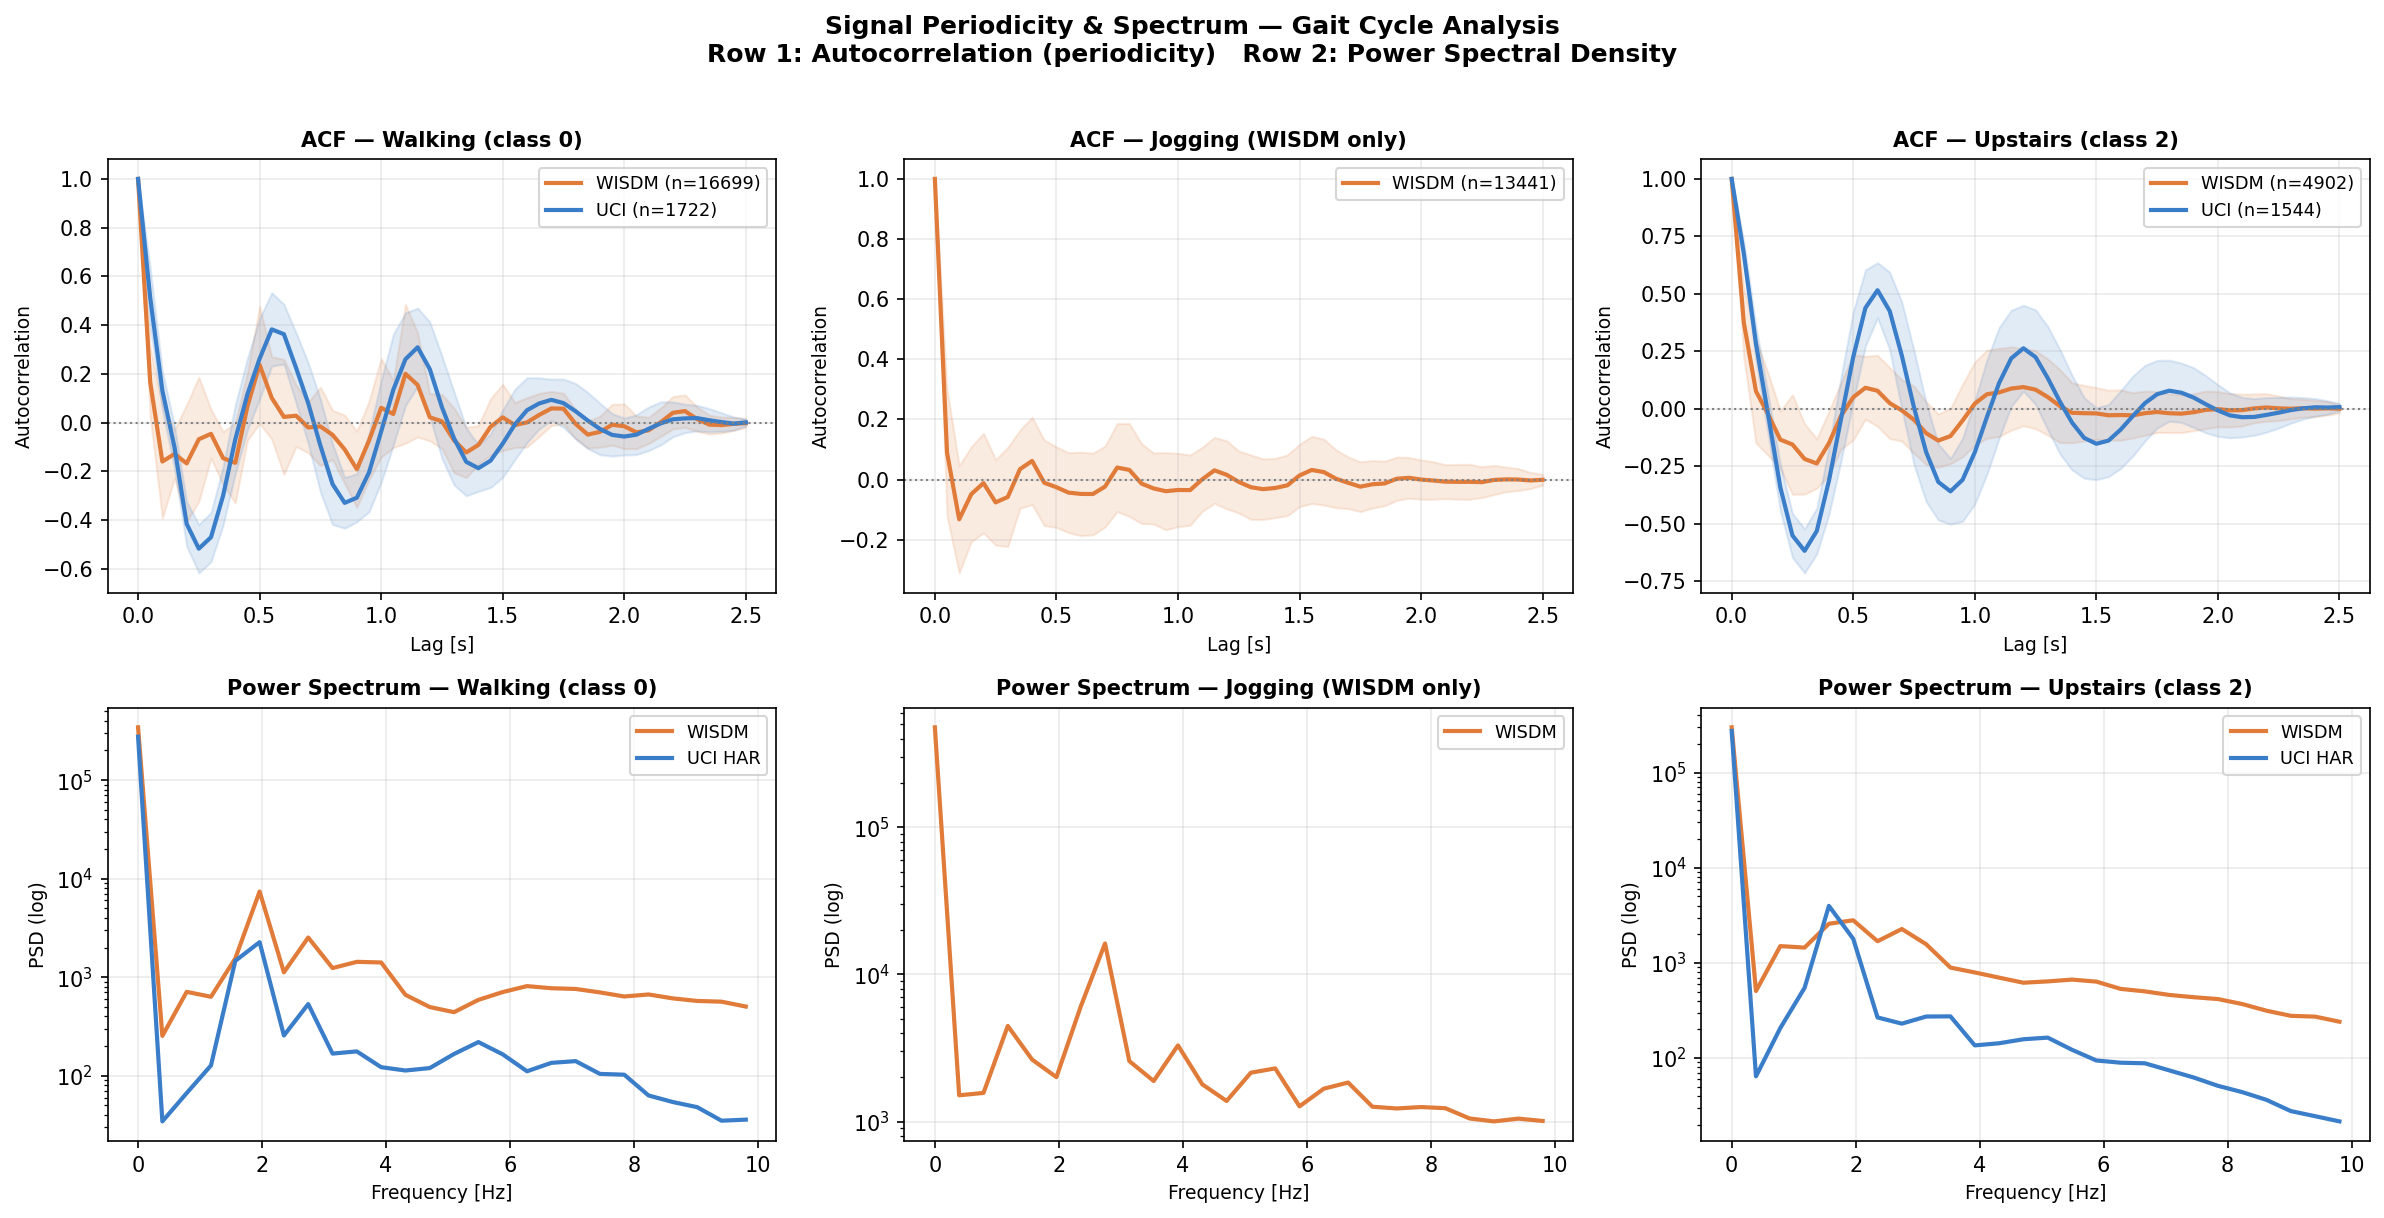
\includegraphics[width=0.90\textwidth, height=0.72\textheight, keepaspectratio]
      {autocorrelation_analysis.png}
  \end{center}
  \vspace{-2mm}
  \begin{center}
    \small \textbf{Row 1:} Autocorrelation — WISDM Walking shows stronger gait periodicity (pocket amplifies step motion) \quad
    \textbf{Row 2:} PSD — WISDM energy concentrated at 1--2 Hz step frequency
  \end{center}
\end{frame}

\begin{frame}{Results Summary — Comprehensive View}
  \begin{center}
    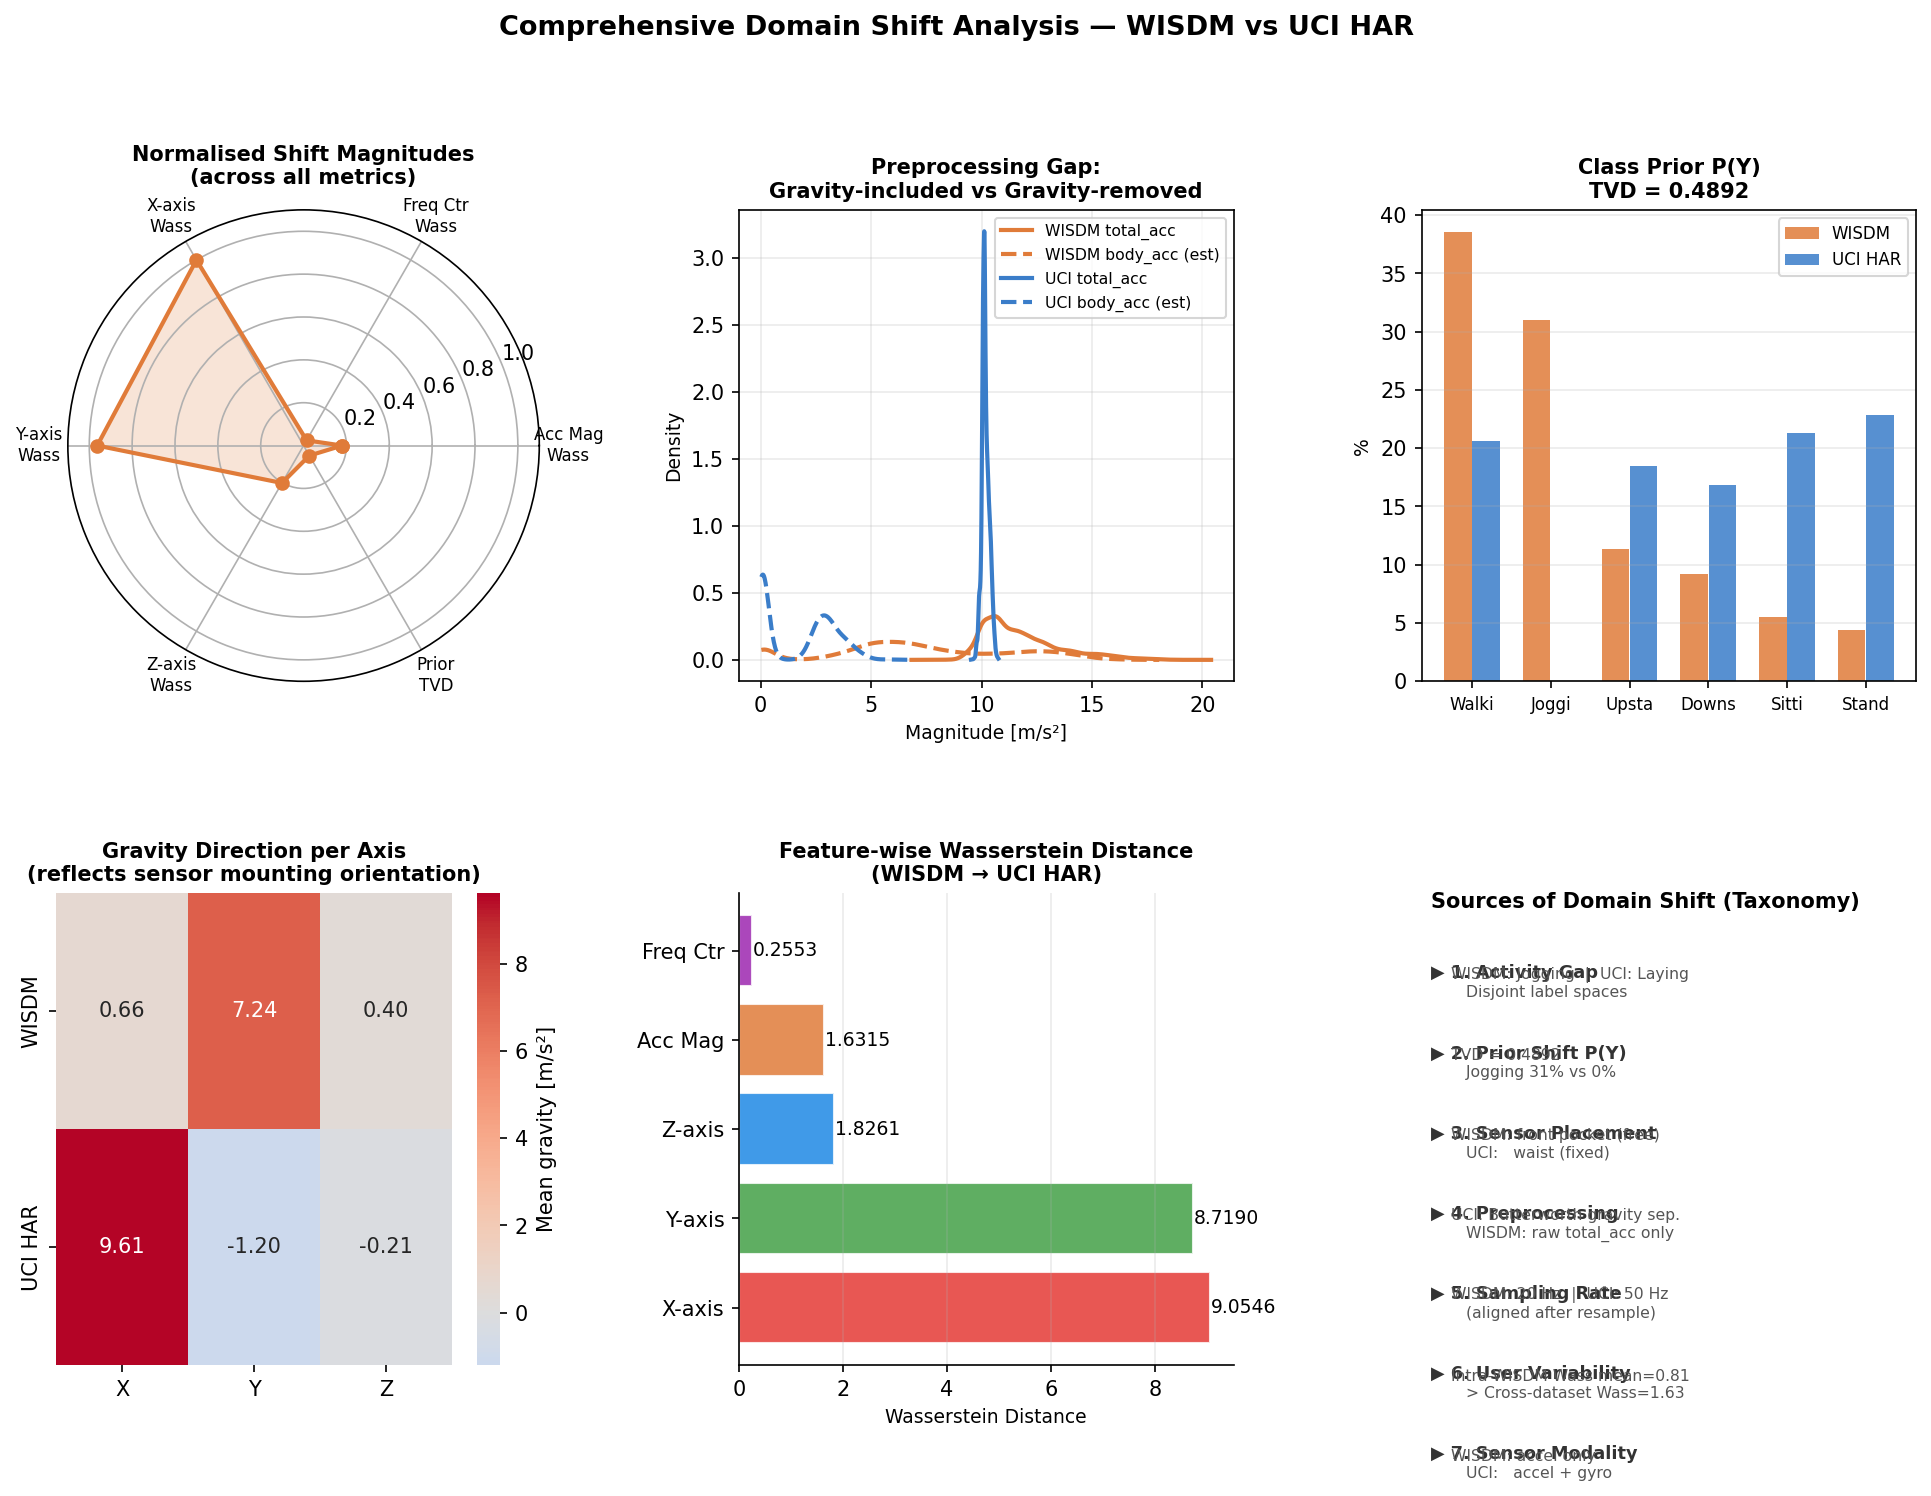
\includegraphics[width=0.90\textwidth, height=0.72\textheight, keepaspectratio]
      {comprehensive_summary.png}
  \end{center}
  \vspace{-1mm}
  \begin{center}
    \small Radar chart confirms: X/Y-axis Wasserstein dominates all other metrics after normalisation
  \end{center}
\end{frame}

\begin{frame}{Metric Summary Table}
  \begin{center}
  \small
  \begin{tabular}{llccc}
    \toprule
    \textbf{Feature / Dimension} & \textbf{Type} & \textbf{Wasserstein} & \textbf{Sym-KL} & \textbf{Note} \\
    \midrule
    \rowcolor{red!10}
    \textbf{X-axis (raw signal)}  & Covariate & \textbf{9.055 m/s²} & 4.647 & Dominant axis \\
    \rowcolor{red!10}
    \textbf{Y-axis (raw signal)}  & Covariate & \textbf{8.719 m/s²} & 4.125 & Dominant axis \\
    Z-axis (raw signal)           & Covariate & 1.826 m/s² & 0.751 & Stable \\
    Acc Magnitude (global)        & Covariate & 1.631 m/s² & 4.653 & Understated \\
    Acc Magnitude — Walking       & Per-class & 1.153 m/s² & 5.617 & Largest class shift \\
    Frequency Centroid            & Covariate & 0.255 Hz   & 3.409 & 5.5$\times$ mean gap \\
    \midrule
    Class Prior TVD               & Prior     & ---         & ---   & \textbf{0.489} \\
    Multi-kernel MMD              & Global    & ---         & ---   & \textbf{0.455} \\
    \rowcolor{yellow!25}
    Max inter-user Wass           & Subject   & \textbf{1.891 m/s²} & --- & $>$ cross-dataset \\
    \bottomrule
  \end{tabular}
  \end{center}
\end{frame}

%% ============================================================
%%  SECTION 5 — CONCLUSIONS
%% ============================================================

\begin{frame}{Seven Sources of Domain Shift — Taxonomy}
  \begin{columns}[T]
    \begin{column}{0.50\textwidth}
      \begin{enumerate}
        \item \textbf{Sensor placement / orientation} \\
              \small X/Y Wass $\approx$ 9 m/s²; gravity projected onto different axes
        \vspace{1mm}
        \item \textbf{Preprocessing pipeline} \\
              \small UCI: Butterworth gravity removal; WISDM: raw total\_acc
        \vspace{1mm}
        \item \textbf{Activity label space mismatch} \\
              \small Jogging (WISDM 31\%) $\leftrightarrow$ Laying (UCI) — no cross-match
        \vspace{1mm}
        \item \textbf{Class prior shift} $P(Y)$ \\
              \small TVD = 0.489
      \end{enumerate}
    \end{column}
    \begin{column}{0.46\textwidth}
      \begin{enumerate}
        \setcounter{enumi}{4}
        \item \textbf{Signal dynamic amplitude} \\
              \small WISDM dynamic std 3--5$\times$ higher across all axes
        \vspace{1mm}
        \item \textbf{Inter-subject variability} \\
              \small Max intra-dataset shift (1.89) $>$ cross-dataset (1.63)
        \vspace{1mm}
        \item \textbf{Sensor modality gap} \\
              \small UCI has gyroscope; WISDM accelerometer only
      \end{enumerate}

      \vspace{4mm}
      \begin{alertblock}{Bottom Line}
        \small Sensor \textbf{orientation} is the dominant shift source — invisible to scalar analysis.
      \end{alertblock}
    \end{column}
  \end{columns}
\end{frame}

\begin{frame}{Recommended Metrics for Cross-Dataset HAR Shift}
  \begin{center}
  \small
  \begin{tabularx}{0.92\textwidth}{llX}
    \toprule
    \textbf{Metric} & \textbf{Captures} & \textbf{When to Use} \\
    \midrule
    \textbf{Per-axis Wasserstein} & Orientation shift & \textbf{Primary metric} — do not use scalar only \\
    Scalar Wasserstein (Acc Mag)  & Magnitude shift   & For comparison with prior literature \\
    Symmetric KL Divergence       & Distributional overlap & Tail sensitivity, shape differences \\
    Multi-kernel MMD              & Global feature-space & Adaptation readiness assessment \\
    Total Variation Distance      & Prior $P(Y)$ shift & Mandatory for imbalanced datasets \\
    Gravity DC analysis           & Orientation / preprocessing & Distinguishes orientation from motion \\
    Inter-user Wasserstein        & Subject heterogeneity & Personalisation difficulty baseline \\
    \bottomrule
  \end{tabularx}
  \end{center}

  \vspace{3mm}
  \begin{block}{Practical Recommendation}
    A complete domain shift characterisation in HAR requires \textbf{all four metric types} (covariate, prior, feature-space, subject-level). Reporting scalar Acc Magnitude shift alone is \textbf{insufficient} and systematically underestimates the true domain gap.
  \end{block}
\end{frame}

\begin{frame}{Conclusions}
  \begin{columns}[T]
    \begin{column}{0.55\textwidth}
      \textbf{Answering the Research Question:}
      \vspace{2mm}
      \begin{itemize}
        \item[\checkmark] \textbf{7 sources} of domain shift identified and quantified
        \item[\checkmark] \textbf{Per-axis analysis} reveals the dominant shift missed by prior work
        \item[\checkmark] \textbf{4 metric classes} cover covariate, prior, feature-space, and subject-level shift
        \item[\checkmark] Intra-dataset user shift can \textbf{exceed} cross-dataset shift
        \item[\checkmark] Preprocessing (gravity separation) is a \textbf{hidden covariate shift} — not just a technicality
      \end{itemize}
    \end{column}

    \begin{column}{0.42\textwidth}
      \begin{block}{Implications for DA Research}
        \begin{itemize}
          \small
          \item Adaptation methods must address sensor \textbf{orientation} explicitly
          \item Standard gravity separation should be applied \textbf{consistently} across datasets
          \item Subject-level adaptation may matter \textbf{more} than dataset-level
          \item Evaluation should report \textbf{per-axis metrics}, not just Acc Mag
        \end{itemize}
      \end{block}

      \vspace{3mm}
      \begin{exampleblock}{Repository}
        \small All code, data, and figures:\\
        \texttt{github.com/gengzhanguo/wisdm\_ucihar}
      \end{exampleblock}
    \end{column}
  \end{columns}
\end{frame}

\begin{frame}[plain]
  \begin{center}
    \vspace{12mm}
    {\Large \textbf{Thank You}}\\[6mm]
    {\normalsize Questions welcome}\\[10mm]
    \textcolor{noteGray}{\small
      All figures, data, and reproducible code available at:\\[2mm]
      \texttt{https://github.com/gengzhanguo/wisdm\_ucihar}
    }\\[12mm]
    \begin{tabular}{cc}
      \textcolor{wisdmOrange}{\textbf{WISDM v1.1}} & \textcolor{uciBlue}{\textbf{UCI HAR}} \\
      Kwapisz et al., 2011 & Anguita et al., 2013
    \end{tabular}
  \end{center}
\end{frame}

\end{document}
